\documentclass[a4paper,dvipdfmx]{jsarticle}
\usepackage{lmodern}
\usepackage[T1]{fontenc}
\usepackage{textcomp}
\usepackage[utf8]{inputenc}
\usepackage{amsmath,amssymb}
\usepackage{inconsolata}
\usepackage{tikz}
\usepackage{okumacro}

\title{Ti{\em k}Zの小さなサンプル}
\author{結城浩\footnote{http://www.hyuki.com/, \texttt{@hyuki}}}
\date{2013年11月10日}

\begin{document}

\maketitle

\begin{center}
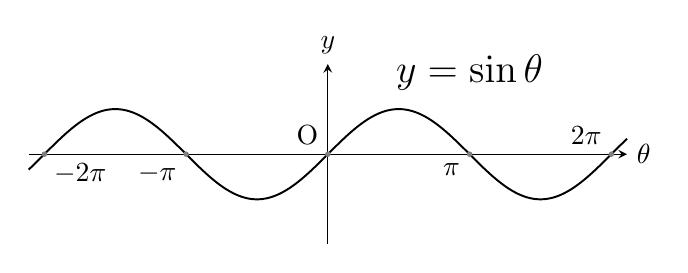
\begin{tikzpicture}[x=0.1mm,y=5.73mm,domain=-380:380,samples=300,>=stealth]
  \draw[->] (-380,0) -- (380,0) node[right] {$\theta$};
  \draw[->] (0,-2) -- (0,2) node[above] {$y$};
  \draw[line width=0.7pt] plot (\x,{sin(\x)});
  \draw plot (180,1.2) node[above] {\Large$y = \sin \theta$};
  \foreach \t in {-360,-180,...,360} \fill[gray] (\t,0) circle (1pt);
  \draw (-360,0) node[below right] {$-2\pi$};
  \draw (-180,0) node[below left]  {$-\pi$};
  \draw (   0,0) node[above left]  {O};
  \draw ( 180,0) node[below left]  {$\pi$};
  \draw ( 360,0) node[above left]  {$2\pi$};
\end{tikzpicture}
\end{center}

\end{document}